

\tikzset{every picture/.style={line width=0.75pt}} %set default line width to 0.75pt        

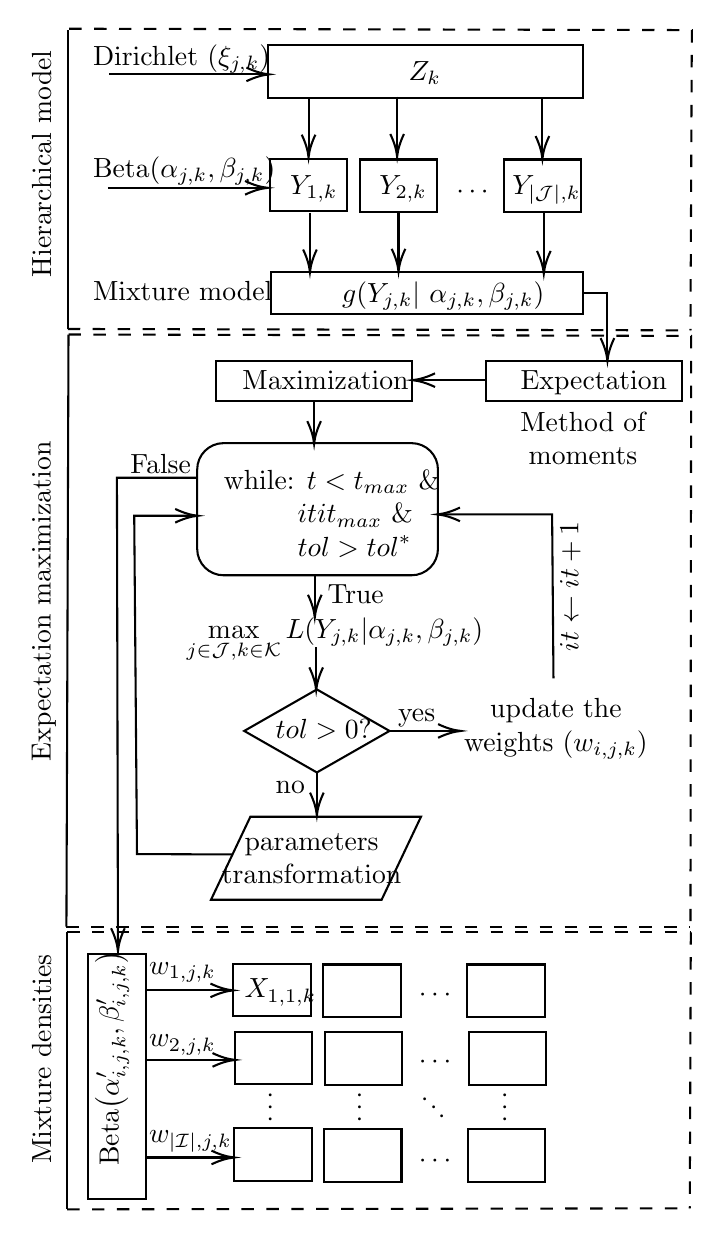
\begin{tikzpicture}[x=0.75pt,y=0.75pt,yscale=-1,xscale=1]
%uncomment if require: \path (0,626); %set diagram left start at 0, and has height of 626

%Shape: Rectangle [id:dp7430473006075338] 
\draw  [color={rgb, 255:red, 0; green, 0; blue, 0 }  ,draw opacity=1 ] (121,31.33) -- (272.33,31.33) -- (272.33,57) -- (121,57) -- cycle ;
%Shape: Rectangle [id:dp4548840073137388] 
\draw  [color={rgb, 255:red, 0; green, 0; blue, 0 }  ,draw opacity=1 ] (121.67,86.33) -- (159,86.33) -- (159,111.67) -- (121.67,111.67) -- cycle ;
%Shape: Rectangle [id:dp9665482146228945] 
\draw  [color={rgb, 255:red, 0; green, 0; blue, 0 }  ,draw opacity=1 ] (122.33,141) -- (272.33,141) -- (272.33,161) -- (122.33,161) -- cycle ;
%Straight Lines [id:da5861777588420125] 
\draw    (43.67,100.33) -- (118.67,100.33) ;
\draw [shift={(120.67,100.33)}, rotate = 180] [color={rgb, 255:red, 0; green, 0; blue, 0 }  ][line width=0.75]    (10.93,-3.29) .. controls (6.95,-1.4) and (3.31,-0.3) .. (0,0) .. controls (3.31,0.3) and (6.95,1.4) .. (10.93,3.29)   ;
%Shape: Rectangle [id:dp888982529226428] 
\draw  [color={rgb, 255:red, 0; green, 0; blue, 0 }  ,draw opacity=1 ] (225.67,183.67) -- (320.33,183.67) -- (320.33,203) -- (225.67,203) -- cycle ;
%Shape: Rectangle [id:dp9592744542009763] 
\draw  [color={rgb, 255:red, 0; green, 0; blue, 0 }  ,draw opacity=1 ] (95.67,183.67) -- (190.33,183.67) -- (190.33,203) -- (95.67,203) -- cycle ;
%Straight Lines [id:da9783477243897578] 
\draw    (225.67,193) -- (192.33,193) ;
\draw [shift={(190.33,193)}, rotate = 360] [color={rgb, 255:red, 0; green, 0; blue, 0 }  ][line width=0.75]    (10.93,-3.29) .. controls (6.95,-1.4) and (3.31,-0.3) .. (0,0) .. controls (3.31,0.3) and (6.95,1.4) .. (10.93,3.29)   ;
%Rounded Rect [id:dp25569846498058046] 
\draw   (86.67,236.07) .. controls (86.67,229.03) and (92.37,223.33) .. (99.4,223.33) -- (189.93,223.33) .. controls (196.97,223.33) and (202.67,229.03) .. (202.67,236.07) -- (202.67,274.27) .. controls (202.67,281.3) and (196.97,287) .. (189.93,287) -- (99.4,287) .. controls (92.37,287) and (86.67,281.3) .. (86.67,274.27) -- cycle ;
%Straight Lines [id:da07746167975332074] 
\draw    (143,203) -- (143,221.67) ;
\draw [shift={(143,223.67)}, rotate = 270] [color={rgb, 255:red, 0; green, 0; blue, 0 }  ][line width=0.75]    (10.93,-3.29) .. controls (6.95,-1.4) and (3.31,-0.3) .. (0,0) .. controls (3.31,0.3) and (6.95,1.4) .. (10.93,3.29)   ;
%Flowchart: Decision [id:dp7428483588855725] 
\draw   (144.33,342) -- (179.33,362) -- (144.33,382) -- (109.33,362) -- cycle ;
%Straight Lines [id:da4514988119896104] 
\draw    (143.33,286.67) -- (143.33,305.33) ;
\draw [shift={(143.33,307.33)}, rotate = 270] [color={rgb, 255:red, 0; green, 0; blue, 0 }  ][line width=0.75]    (10.93,-3.29) .. controls (6.95,-1.4) and (3.31,-0.3) .. (0,0) .. controls (3.31,0.3) and (6.95,1.4) .. (10.93,3.29)   ;
%Straight Lines [id:da7225713548898394] 
\draw    (144,321.67) -- (144,340.33) ;
\draw [shift={(144,342.33)}, rotate = 270] [color={rgb, 255:red, 0; green, 0; blue, 0 }  ][line width=0.75]    (10.93,-3.29) .. controls (6.95,-1.4) and (3.31,-0.3) .. (0,0) .. controls (3.31,0.3) and (6.95,1.4) .. (10.93,3.29)   ;
%Flowchart: Data [id:dp01613550529518437] 
\draw   (112.3,403.33) -- (194.5,403.33) -- (175.53,443.33) -- (93.33,443.33) -- cycle ;
%Straight Lines [id:da8047561439582993] 
\draw    (144.33,382) -- (144.33,400.67) ;
\draw [shift={(144.33,402.67)}, rotate = 270] [color={rgb, 255:red, 0; green, 0; blue, 0 }  ][line width=0.75]    (10.93,-3.29) .. controls (6.95,-1.4) and (3.31,-0.3) .. (0,0) .. controls (3.31,0.3) and (6.95,1.4) .. (10.93,3.29)   ;
%Straight Lines [id:da05391313938609321] 
\draw    (103.5,421.5) -- (57.67,421.33) -- (56.33,258.33) -- (85,258.33) ;
\draw [shift={(87,258.33)}, rotate = 180] [color={rgb, 255:red, 0; green, 0; blue, 0 }  ][line width=0.75]    (10.93,-3.29) .. controls (6.95,-1.4) and (3.31,-0.3) .. (0,0) .. controls (3.31,0.3) and (6.95,1.4) .. (10.93,3.29)   ;
%Straight Lines [id:da5822221678252375] 
\draw    (179.33,362) -- (211.67,362) ;
\draw [shift={(213.67,362)}, rotate = 180] [color={rgb, 255:red, 0; green, 0; blue, 0 }  ][line width=0.75]    (10.93,-3.29) .. controls (6.95,-1.4) and (3.31,-0.3) .. (0,0) .. controls (3.31,0.3) and (6.95,1.4) .. (10.93,3.29)   ;
%Straight Lines [id:da12553420804327753] 
\draw    (258.33,336.67) -- (257.67,257.67) -- (204.33,257.67) ;
\draw [shift={(202.33,257.67)}, rotate = 360] [color={rgb, 255:red, 0; green, 0; blue, 0 }  ][line width=0.75]    (10.93,-3.29) .. controls (6.95,-1.4) and (3.31,-0.3) .. (0,0) .. controls (3.31,0.3) and (6.95,1.4) .. (10.93,3.29)   ;
%Shape: Rectangle [id:dp3247112292270131] 
\draw  [color={rgb, 255:red, 0; green, 0; blue, 0 }  ,draw opacity=1 ] (165,86.67) -- (202.33,86.67) -- (202.33,112) -- (165,112) -- cycle ;
%Shape: Rectangle [id:dp1315376782374127] 
\draw  [color={rgb, 255:red, 0; green, 0; blue, 0 }  ,draw opacity=1 ] (234.33,86.67) -- (271.67,86.67) -- (271.67,112) -- (234.33,112) -- cycle ;
%Straight Lines [id:da8759399514910455] 
\draw    (141,112.33) -- (141,139) ;
\draw [shift={(141,141)}, rotate = 270] [color={rgb, 255:red, 0; green, 0; blue, 0 }  ][line width=0.75]    (10.93,-3.29) .. controls (6.95,-1.4) and (3.31,-0.3) .. (0,0) .. controls (3.31,0.3) and (6.95,1.4) .. (10.93,3.29)   ;
%Straight Lines [id:da68075728646023] 
\draw    (183.67,111.67) -- (183.67,138.67) ;
\draw [shift={(183.67,140.67)}, rotate = 270] [color={rgb, 255:red, 0; green, 0; blue, 0 }  ][line width=0.75]    (10.93,-3.29) .. controls (6.95,-1.4) and (3.31,-0.3) .. (0,0) .. controls (3.31,0.3) and (6.95,1.4) .. (10.93,3.29)   ;
%Straight Lines [id:da4828595520010639] 
\draw    (253.67,112.33) -- (253.67,139.67) ;
\draw [shift={(253.67,141.67)}, rotate = 270] [color={rgb, 255:red, 0; green, 0; blue, 0 }  ][line width=0.75]    (10.93,-3.29) .. controls (6.95,-1.4) and (3.31,-0.3) .. (0,0) .. controls (3.31,0.3) and (6.95,1.4) .. (10.93,3.29)   ;
%Straight Lines [id:da8284525040523023] 
\draw    (272.33,151) -- (284.33,151) -- (284.33,181.67) ;
\draw [shift={(284.33,183.67)}, rotate = 270] [color={rgb, 255:red, 0; green, 0; blue, 0 }  ][line width=0.75]    (10.93,-3.29) .. controls (6.95,-1.4) and (3.31,-0.3) .. (0,0) .. controls (3.31,0.3) and (6.95,1.4) .. (10.93,3.29)   ;
%Straight Lines [id:da2256320384343773] 
\draw    (140.33,57) -- (140.33,83.67) ;
\draw [shift={(140.33,85.67)}, rotate = 270] [color={rgb, 255:red, 0; green, 0; blue, 0 }  ][line width=0.75]    (10.93,-3.29) .. controls (6.95,-1.4) and (3.31,-0.3) .. (0,0) .. controls (3.31,0.3) and (6.95,1.4) .. (10.93,3.29)   ;
%Straight Lines [id:da38126124094165625] 
\draw    (183,56.33) -- (183,83.33) ;
\draw [shift={(183,85.33)}, rotate = 270] [color={rgb, 255:red, 0; green, 0; blue, 0 }  ][line width=0.75]    (10.93,-3.29) .. controls (6.95,-1.4) and (3.31,-0.3) .. (0,0) .. controls (3.31,0.3) and (6.95,1.4) .. (10.93,3.29)   ;
%Straight Lines [id:da8300332483567019] 
\draw    (253,57) -- (253,84.33) ;
\draw [shift={(253,86.33)}, rotate = 270] [color={rgb, 255:red, 0; green, 0; blue, 0 }  ][line width=0.75]    (10.93,-3.29) .. controls (6.95,-1.4) and (3.31,-0.3) .. (0,0) .. controls (3.31,0.3) and (6.95,1.4) .. (10.93,3.29)   ;
%Straight Lines [id:da35166778374890373] 
\draw    (44.33,45.67) -- (119.33,45.67) ;
\draw [shift={(121.33,45.67)}, rotate = 180] [color={rgb, 255:red, 0; green, 0; blue, 0 }  ][line width=0.75]    (10.93,-3.29) .. controls (6.95,-1.4) and (3.31,-0.3) .. (0,0) .. controls (3.31,0.3) and (6.95,1.4) .. (10.93,3.29)   ;
%Straight Lines [id:da6418466816634409] 
\draw    (24.67,171) -- (23.67,456.33) ;
%Straight Lines [id:da4486614945554752] 
\draw    (24.33,24.33) -- (24.33,168.33) ;
%Straight Lines [id:da3901477778136966] 
\draw  [dash pattern={on 4.5pt off 4.5pt}]  (24.33,168.33) -- (324.33,169) ;
%Straight Lines [id:da7411545386420908] 
\draw  [dash pattern={on 4.5pt off 4.5pt}]  (24.67,171) -- (324.67,171.67) -- (324.33,456.33) ;
%Straight Lines [id:da57228337026407] 
\draw  [dash pattern={on 4.5pt off 4.5pt}]  (23.67,456.33) -- (324.33,456.33) ;
%Straight Lines [id:da18551112028253502] 
\draw  [dash pattern={on 4.5pt off 4.5pt}]  (25,23.67) -- (325,24.33) -- (324.33,169) ;
%Shape: Rectangle [id:dp9694721320590864] 
\draw  [color={rgb, 255:red, 0; green, 0; blue, 0 }  ,draw opacity=1 ] (104.1,474.2) -- (141.43,474.2) -- (141.43,499.53) -- (104.1,499.53) -- cycle ;
%Shape: Rectangle [id:dp7444561338712485] 
\draw  [color={rgb, 255:red, 0; green, 0; blue, 0 }  ,draw opacity=1 ] (147.43,474.53) -- (184.77,474.53) -- (184.77,499.87) -- (147.43,499.87) -- cycle ;
%Shape: Rectangle [id:dp6817699559972299] 
\draw  [color={rgb, 255:red, 0; green, 0; blue, 0 }  ,draw opacity=1 ] (216.77,474.53) -- (254.1,474.53) -- (254.1,499.87) -- (216.77,499.87) -- cycle ;
%Shape: Rectangle [id:dp42575946454884583] 
\draw  [color={rgb, 255:red, 0; green, 0; blue, 0 }  ,draw opacity=1 ] (104.77,506.87) -- (142.1,506.87) -- (142.1,532.2) -- (104.77,532.2) -- cycle ;
%Shape: Rectangle [id:dp25188440840595216] 
\draw  [color={rgb, 255:red, 0; green, 0; blue, 0 }  ,draw opacity=1 ] (148.1,507.2) -- (185.43,507.2) -- (185.43,532.53) -- (148.1,532.53) -- cycle ;
%Shape: Rectangle [id:dp1957750462964596] 
\draw  [color={rgb, 255:red, 0; green, 0; blue, 0 }  ,draw opacity=1 ] (217.43,507.2) -- (254.77,507.2) -- (254.77,532.53) -- (217.43,532.53) -- cycle ;
%Shape: Rectangle [id:dp858540062713069] 
\draw  [color={rgb, 255:red, 0; green, 0; blue, 0 }  ,draw opacity=1 ] (104.43,553.51) -- (141.77,553.51) -- (141.77,578.84) -- (104.43,578.84) -- cycle ;
%Shape: Rectangle [id:dp9224366389369734] 
\draw  [color={rgb, 255:red, 0; green, 0; blue, 0 }  ,draw opacity=1 ] (147.77,553.84) -- (185.1,553.84) -- (185.1,579.18) -- (147.77,579.18) -- cycle ;
%Shape: Rectangle [id:dp7020980735854778] 
\draw  [color={rgb, 255:red, 0; green, 0; blue, 0 }  ,draw opacity=1 ] (217.1,553.84) -- (254.43,553.84) -- (254.43,579.18) -- (217.1,579.18) -- cycle ;
%Straight Lines [id:da09761708626685728] 
\draw    (62,487) -- (102,487) ;
\draw [shift={(104,487)}, rotate = 180] [color={rgb, 255:red, 0; green, 0; blue, 0 }  ][line width=0.75]    (10.93,-3.29) .. controls (6.95,-1.4) and (3.31,-0.3) .. (0,0) .. controls (3.31,0.3) and (6.95,1.4) .. (10.93,3.29)   ;
%Straight Lines [id:da8630702615768855] 
\draw    (61.5,520.5) -- (103,520.5) ;
\draw [shift={(105,520.5)}, rotate = 180] [color={rgb, 255:red, 0; green, 0; blue, 0 }  ][line width=0.75]    (10.93,-3.29) .. controls (6.95,-1.4) and (3.31,-0.3) .. (0,0) .. controls (3.31,0.3) and (6.95,1.4) .. (10.93,3.29)   ;
%Straight Lines [id:da08239644065275953] 
\draw    (86,240) -- (48,240) -- (48.5,466) ;
\draw [shift={(48.5,468)}, rotate = 269.87] [color={rgb, 255:red, 0; green, 0; blue, 0 }  ][line width=0.75]    (10.93,-3.29) .. controls (6.95,-1.4) and (3.31,-0.3) .. (0,0) .. controls (3.31,0.3) and (6.95,1.4) .. (10.93,3.29)   ;
%Shape: Rectangle [id:dp04261132612453555] 
\draw   (34,469.5) -- (62,469.5) -- (62,587.5) -- (34,587.5) -- cycle ;
%Straight Lines [id:da03789465017191529] 
\draw    (62.5,567.5) -- (102.5,567.5) ;
\draw [shift={(104.5,567.5)}, rotate = 180] [color={rgb, 255:red, 0; green, 0; blue, 0 }  ][line width=0.75]    (10.93,-3.29) .. controls (6.95,-1.4) and (3.31,-0.3) .. (0,0) .. controls (3.31,0.3) and (6.95,1.4) .. (10.93,3.29)   ;
%Straight Lines [id:da7922516760292679] 
\draw    (24,459) -- (24,592.5) ;
%Straight Lines [id:da4296479621688276] 
\draw  [dash pattern={on 4.5pt off 4.5pt}]  (24,459) -- (324.5,459) ;
%Straight Lines [id:da38093508049365643] 
\draw  [dash pattern={on 4.5pt off 4.5pt}]  (324.5,459) -- (324,592) ;
%Straight Lines [id:da5175247853651179] 
\draw  [dash pattern={on 4.5pt off 4.5pt}]  (24,592.5) -- (324,592) ;

% Text Node
\draw (35,30) node [anchor=north west][inner sep=0.75pt]   [align=left] {Dirichlet ($\displaystyle \xi _{j,k}$)};
% Text Node
\draw (187,38) node [anchor=north west][inner sep=0.75pt]   [align=left] {$\displaystyle Z_{k}$};
% Text Node
\draw (155,144) node [anchor=north west][inner sep=0.75pt]   [align=left] {$\displaystyle g( Y_{j,k} |\ \alpha _{j,k} ,\beta _{j,k})$};
% Text Node
\draw (130,93) node [anchor=north west][inner sep=0.75pt]   [align=left] {$\displaystyle Y_{1,k}$};
% Text Node
\draw (35,84) node [anchor=north west][inner sep=0.75pt]   [align=left] {Beta$\displaystyle ( \alpha _{j,k} ,\beta _{j,k})$};
% Text Node
\draw (241,187) node [anchor=north west][inner sep=0.75pt]   [align=left] {Expectation};
% Text Node
\draw (239,207) node [anchor=north west][inner sep=0.75pt]   [align=left] {\begin{minipage}[lt]{48.088784000000004pt}\setlength\topsep{0pt}
\begin{center}
Method of\\moments
\end{center}

\end{minipage}};
% Text Node
\draw (80,306) node [anchor=north west][inner sep=0.75pt]   [align=left] {$\displaystyle \max_{j \in \mathcal{J},k \in \mathcal{K}} L( Y_{j,k} |\alpha _{j,k} ,\beta _{j,k})$};
% Text Node
\draw (107,187) node [anchor=north west][inner sep=0.75pt]   [align=left] {Maximization};
% Text Node
\draw (98,235) node [anchor=north west][inner sep=0.75pt]   [align=left] {while: $\displaystyle t< t_{max}$ \&\\ \ \ \ \ \ \ \ \ $\displaystyle it\leqslant it_{max}$ \&\\ \ \ \ \ \ \ \ \ $\displaystyle tol >tol^{*}$};
% Text Node
\draw (123,355) node [anchor=north west][inner sep=0.75pt]   [align=left] {$\displaystyle tol >0$?};
% Text Node
\draw (95,410) node [anchor=north west][inner sep=0.75pt]   [align=left] {\begin{minipage}[lt]{67.915pt}\setlength\topsep{0pt}
\begin{center}
parameters\\transformation
\end{center}

\end{minipage}};
% Text Node
\draw (123,385) node [anchor=north west][inner sep=0.75pt]   [align=left] {no};
% Text Node
\draw (182,350) node [anchor=north west][inner sep=0.75pt]   [align=left] {yes};
% Text Node
\draw (212,345) node [anchor=north west][inner sep=0.75pt]   [align=left] {\begin{minipage}[lt]{69.02000000000001pt}\setlength\topsep{0pt}
\begin{center}
update the\\weights ($\displaystyle w_{i,j,k}$)
\end{center}

\end{minipage}};
% Text Node
\draw (260,325) node [anchor=north west][inner sep=0.75pt]  [rotate=-269.98] [align=left] {$\displaystyle it\leftarrow it+1$};
% Text Node
\draw (173,93) node [anchor=north west][inner sep=0.75pt]   [align=left] {$\displaystyle Y_{2,k}$};
% Text Node
\draw (237,93) node [anchor=north west][inner sep=0.75pt]   [align=left] {$\displaystyle Y_{|\mathcal{J}|,k}$};
% Text Node
\draw (210,98) node [anchor=north west][inner sep=0.75pt]   [align=left] {$\displaystyle \cdots $};
% Text Node
\draw (35,144) node [anchor=north west][inner sep=0.75pt]   [align=left] {Mixture model};
% Text Node
\draw (5.5,145) node [anchor=north west][inner sep=0.75pt]  [rotate=-270] [align=left] {Hierarchical model};
% Text Node
\draw (5.5,378) node [anchor=north west][inner sep=0.75pt]  [rotate=-270] [align=left] {Expectation maximization};
% Text Node
\draw (148,290) node [anchor=north west][inner sep=0.75pt]   [align=left] {True};
% Text Node
\draw (108,480) node [anchor=north west][inner sep=0.75pt]   [align=left] {$\displaystyle X_{1,1,k}$};
% Text Node
\draw (151,480) node [anchor=north west][inner sep=0.75pt]   [align=left] {};
% Text Node
\draw (192,485) node [anchor=north west][inner sep=0.75pt]   [align=left] {$\displaystyle \cdots $};
% Text Node
\draw (216,480) node [anchor=north west][inner sep=0.75pt]   [align=left] {};
% Text Node
\draw (108,512) node [anchor=north west][inner sep=0.75pt]   [align=left] {};
% Text Node
\draw (151,512) node [anchor=north west][inner sep=0.75pt]   [align=left] {};
% Text Node
\draw (192,517) node [anchor=north west][inner sep=0.75pt]   [align=left] {$\displaystyle \cdots $};
% Text Node
\draw (216,512) node [anchor=north west][inner sep=0.75pt]   [align=left] {};
% Text Node
\draw (126,534) node [anchor=north west][inner sep=0.75pt]  [rotate=-90] [align=left] {$\displaystyle \cdots $};
% Text Node
\draw (104,560) node [anchor=north west][inner sep=0.75pt]   [align=left] {};
% Text Node
\draw (147,560) node [anchor=north west][inner sep=0.75pt]   [align=left] {};
% Text Node
\draw (192,565) node [anchor=north west][inner sep=0.75pt]   [align=left] {$\displaystyle \cdots $};
% Text Node
\draw (215,560) node [anchor=north west][inner sep=0.75pt]   [align=left] {};
% Text Node
\draw (169,534) node [anchor=north west][inner sep=0.75pt]  [rotate=-90] [align=left] {$\displaystyle \cdots $};
% Text Node
\draw (239,534) node [anchor=north west][inner sep=0.75pt]  [rotate=-90] [align=left] {$\displaystyle \cdots $};
% Text Node
\draw (197,534) node [anchor=north west][inner sep=0.75pt]  [rotate=-45] [align=left] {$\displaystyle \cdots $};
% Text Node
\draw (53,227) node [anchor=north west][inner sep=0.75pt]   [align=left] {False};
% Text Node
\draw (36,573) node [anchor=north west][inner sep=0.75pt]  [rotate=-270] [align=left] {Beta$\displaystyle \left( \alpha ^{\prime }_{i,j,k} ,\beta ^{\prime }_{i,j,k}\right)$};
% Text Node
\draw (62,472) node [anchor=north west][inner sep=0.75pt]   [align=left] {$\displaystyle w_{1,j,k}$};
% Text Node
\draw (62,507) node [anchor=north west][inner sep=0.75pt]   [align=left] {$\displaystyle w_{2,j,k}$};
% Text Node
\draw (62,553) node [anchor=north west][inner sep=0.75pt]   [align=left] {$\displaystyle w_{|\mathcal{I}|,j,k}$};
% Text Node
\draw (5.5,572) node [anchor=north west][inner sep=0.75pt]  [rotate=-270] [align=left] {Mixture densities};


\end{tikzpicture}
